\documentclass[DM,toc]{lsstdoc}
\usepackage{booktabs}

\title[Qserv Test Summer 2015]{Qserv Summer 15 Large Scale Tests}
\author{Jacek~Becla}
\date{2015-08-27}
\setDocRef{DMTR-13}

\setDocAbstract{%
This document captures information about the large scale tests we ran on the IN2P3 cluster during Summer 2015.

For comparisons, the previous large scale test can be found in \citeds{DMTR-12}.
}

\begin{document}
\maketitle


\section{Data Set}\label{data-set}

\begin{longtable}[]{@{}llll@{}}
\toprule
\textbf{table} & \textbf{row count} & \textbf{.MYD size {[}TB{]}} &
\textbf{.MYI size {[}TB{]}}\tabularnewline
\midrule
\endhead
Object & 1,889,695,615 & ~2.45 & 0.06\tabularnewline
Source & 34,886,017,763 & 17.13 & 2.05\tabularnewline
ForcedSource & 172,081,115,270` & 5.85 & 4.61\tabularnewline
\bottomrule
\end{longtable}

~

Total MySQL data dir size: 33.2 TB

So for Object and Source we are at the \textasciitilde{}10\% of DR1
level. We have more Forced Sources than 10\% of DR1.

\section{Hardware}\label{hardware}

\begin{itemize}
\item
  50 nodes, DELL PowerEdge R620
\item
  2 x Processors Intel Xeon E5-2603v2 @ 1.80 Ghz 4 core
\item
  10 Mo cache, 6.4 GT/s, 80W
\item
  Memory 16 GB DDR-3 @ 1600MHz (2x8GB)
\item
  2 x hard drive 250GB SATA 7200 Rpm 2,5" - hotplug =\textgreater{} OS
\item
  8 x hard drive 1 TB Nearline SAS 6 Gbps 7200 Rpm 2,5"
\item
  hotplug =\textgreater{} DATA
\item
  1 x card RAID H710p with 1 GB nvram
\item
  1 x card1 GbE 4 ports Broadcom® 5720 Base-T
\item
  1 x card iDRAC 7 Enterprise
\end{itemize}

\section{Timing summary}\label{timing-summary}

Data on 24 nodes (for comparison, DR1 is expected to be on~92 nodes).

~

\subsection{\texorpdfstring{\textbf{Short
queries}}{Short queries}}\label{short-queries}

\begin{itemize}
\item
  single object selection by id: 0.09 sec
\item
  small spatial area selection from Object: 0.33 sec
\end{itemize}

\subsection{\texorpdfstring{\textbf{Full table scans, single query at
a
time}}{Full table scans, single query at a time}}\label{full-table-scans-single-query-at-a-time}

\begin{itemize}
\item
  Object \textasciitilde{}4 min
\item
  Source \textasciitilde{}18 min
\item
  ForcedSource \textasciitilde{}15 min
\end{itemize}

\subsection{\texorpdfstring{\textbf{Full table joins, single query at
a
time}}{Full table joins, single query at a time}}\label{full-table-joins-single-query-at-a-time}

\begin{itemize}
\item
  Object x Source: \textasciitilde{}23 min
\item
  Object x ForcedSource: \textasciitilde{} 21 min
\end{itemize}

\subsection{\texorpdfstring{\textbf{Concurrent
scans}}{Concurrent scans}}\label{concurrent-scans}

\begin{itemize}
\item
  2 Object scans \textasciitilde{} 8 min, ~5 Object scans
  \textasciitilde{}16-20 min~(this shows that our shared scan code has
  issues, scheduled to be solved in W16)
\end{itemize}

\subsection{\texorpdfstring{\textbf{\emph{Heavy load test 50 LV + 5
HV}}}{Heavy load test 50 LV + 5 HV}}\label{heavy-load-test-50-lv-5-hv}

\begin{itemize}
\item
  50 low volume and 5 high volume queries (3 scans for Object, 1 scan
  for Source, 1 Object-Source joins), all running simultaneously with
  appropriate sleep in between queries to enforce the mix we were aiming
\item
  During 24 hours we completed:

  \begin{itemize}
  \item
    431,597 low volume queries (consistent with the baseline:
    \textasciitilde{}10 sec per query, or 432,000 queries in 24h)
  \item
    73 Object scans (consistent with baseline: \textasciitilde{}1h per
    query, or 72 in 24h)
  \item
    3 Source scans (consistent with baseline: \textasciitilde{}8h per
    query, or 3 in 24h)
  \item
    3 Object-Source joins (consistent with the baseline
    \textasciitilde{}8h per query, or 3 in 24h)
  \item
    overall size of results was 6.5 GB (\textasciitilde{}16 KB per query
    on average)
  \end{itemize}
\item
  Average times:

  \begin{itemize}
  \item
    low volume queries: 0.91 sec (per baseline, should be under 10 sec)
  \item
    Object scan: 15 min (per baseline, should be under 1 hour)
  \item
    Source scan: 56 min (per baseline, should be under 8 hours)
  \item
    Object-Source join 57 min (per baseline, should be under 8 hours)
  \end{itemize}
\item
  Observations:

  \begin{itemize}
  \item
    io bound during the time when scans happen at the same time. Disks
    85-90\% busy (\textasciitilde{}750 MB/sec seen)
  \item
    the aggregate load on the
    cluster is shown in Fig~\ref{fig:aggload5}.
  \end{itemize}
\end{itemize}

\begin{figure}
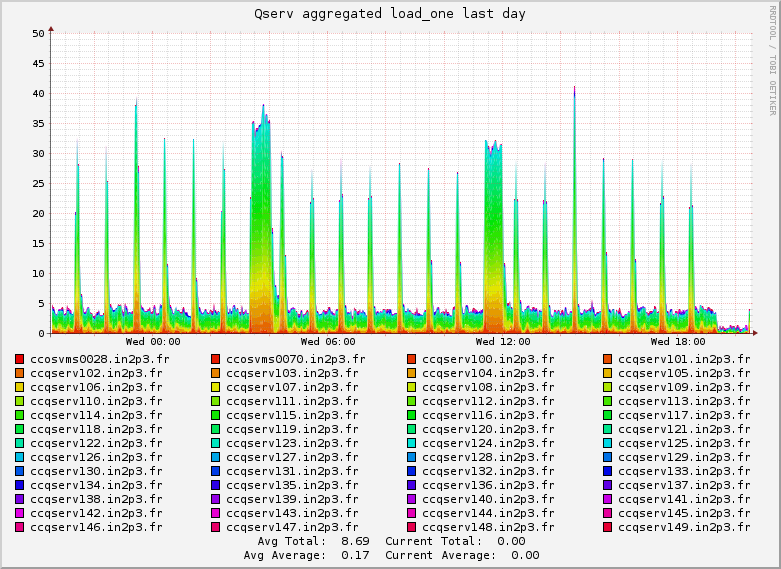
\includegraphics[width=\textwidth]{in2p3_5HV50LV}
\caption{Aggregate load on cluster during heavy load test 50LV + 5HV.}
\label{fig:aggload5}
\end{figure}

\subsection{\texorpdfstring{\textbf{\emph{Heavy load test 100 LV + 10
HV}}}{Heavy load test 100 LV + 10 HV}}\label{heavy-load-test-100-lv-10-hv}

\begin{itemize}
\item
  100 low volume and 10 high volume queries (6 scans for Object, 2 scan
  for Source, 2 Object-Source joins), all running simultaneously with
  appropriate sleep in between queries to enforce the mix we were aiming
\item
  During 24 hours we completed:

  \begin{itemize}
  \item
    861,608 low volume queries
  \item
    144 Object scans
  \item
    6 Source scans
  \item
    8 Object-Source joins
  \end{itemize}
\item
  Average times:

  \begin{itemize}
  \item
    low volume queries:~5.1 sec
  \item
    Object scan: 22 min
  \item
    Source scan: ~1 h 33 min
  \item
    Object-Source join 1 h 22 min
  \end{itemize}
\item
  Observations:

  \begin{itemize}
  \item
    the aggregate load on the
    cluster is shown in Fig.~\ref{fig:aggload10}.
  \end{itemize}
\item
  Notes: during the last part of that test we were reloading data on the
  node ccqserv101, which was impacted how the average load on the
  cluster looked like
\end{itemize}

\begin{figure}
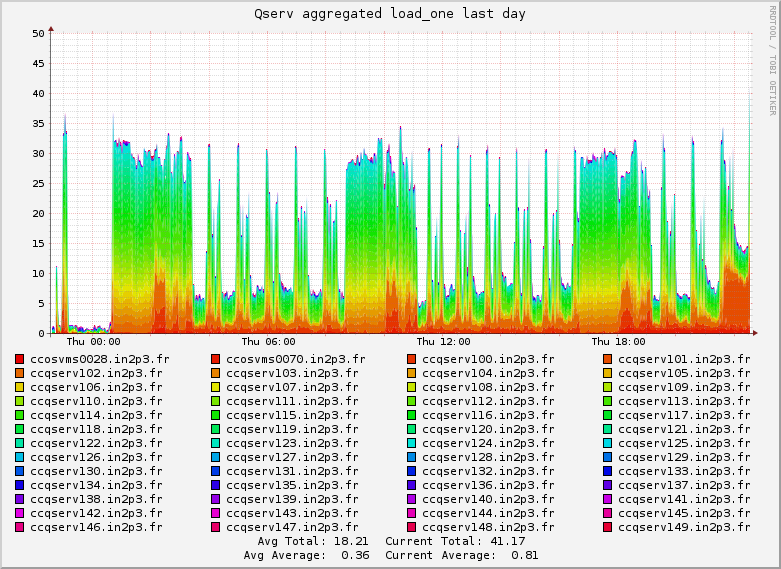
\includegraphics[width=\textwidth]{in2p3_10HV100LV}
\caption{Aggregate load on cluster during heavy load test 100LV + 10HV.}
\label{fig:aggload10}
\end{figure}


\section{Notes and Observations}\label{notes-and-observations}

\begin{itemize}
\item
  \emph{Concurrently greatly improved}. This was the very first time we
  ever successfully ran more than 3-4 simultaneous queries (we run up to
  110).
\item
  \emph{Robustness greatly improved}. This was the very first time we
  ran continuously without any failure for 24 hours (it could have ran
  for longer, we just limited it to 24h)
\item
  \emph{Latency reduced 100x}. In previous tests average time to
  complete low-volume query was above 1 sec. Some of the latest
  improvements involve reducing latency, in particular the overhead of
  query dispatch and sending back result data. The improvements are
  clearly visible, we were able to demonstrate 90 milisec response time
  for individual low-volume queries - 100x better than before.
\item
  Work to do:

  \begin{itemize}
  \item
    When we run 5 full scan queries, some low volume queries get stuck,
    and wait to be scheduled for a long time (minutes), this needs to be
    optimized. But overall things balance out because full scan queries
    end before planned time and there is quite time, when low volume
    queries can catch up.
  \item
    Single-table scared scans are not working well. This will be fixed
    in W16
  \item
    Multi-node shared scans are not working. We did not implement it
    yet. The plan is to implement this in W16
  \item
    The tests revealed problem with handling large results on the master
    node: when a query involves multi-GB results, our master node will
    currently use excessive amount of memory and CPU. (Some of the tests
    we ran produced result sets up to 46 GB over the period of 30
    hours). The uncovered issue will be addressed in FY16 (%
    \href{https://jira.lsstcorp.org/browse/DM-3495}{DM-3495})~
  \end{itemize}
\end{itemize}

\section{Sample Queries}\label{sample-queries}

The actual program that we used to drive the testing can be found
at:~\href{https://github.com/lsst-dm/db_tests_summer15/blob/tickets/DM-3364/DM-3364/runQueries.py}{runQueries.py}

Trivial query that retrieves one row, using index

SELECT * FROM Object WHERE objectId = \textless{}objId\textgreater{}

Counts

SELECT COUNT( * )~FROM Object

SELECT COUNT( * )~FROM Source

SELECT COUNT( * )~FROM ForcedSource

Spatially restricted query, small area of sky, should return small
number of rows (say \textless{}100)

SELECT COUNT( * )\\
FROM Object\\
WHERE ra\_PS BETWEEN 1 AND 2\\
AND decl\_PS BETWEEN 3 AND 4\\
\{quote\}

Full table scan, use some column in WHERE that is not indexes, make sure
the number of results returned is sane (eg thousands, not millions)

SELECT objectId, ra\_PS, decl\_PS, \textless{}few other
columns\textgreater{}\\
FROM Object\\
WHERE fluxToAbMag(iFlux\_PS) - fluxToAbMag(zFlux\_PS) \textgreater{} 4

Aggregation

SELECT COUNT(*) AS n,\\
AVG(ra\_PS),\\
AVG(decl\_PS), chunkId\\
FROM Object\\
GROUP BY chunkId

Near neighbor

SELECT COUNT(*)\\
FROM Object o1, Object o2\\
WHERE qserv\_areaspec\_box(-5,-5,5,-5)\\
AND qserv\_angSep(o1.ra\_PS, o1.decl\_PS, o2.ra\_PS, o2.decl\_PS)
\textless{} 0.1

Joins

SELECT o.objectId, s.sourceId, ra\_PS, decl\_PS, \textless{}few other
columns\textgreater{}\\
FROM Object\\
JOIN SOURCE USING (objectId)\\
WHERE fluxToAbMag(iFlux\_PS) - fluxToAbMag(zFlux\_PS) \textgreater{} 4\\
AND \textless{}some restriction from source table\textgreater{}~

\section{Raw output from selected individual
queries}\label{raw-output-from-selected-individual-queries}

Numbers for 24h scaling tests not shown due to size of the output

\subsection{Counts}\label{counts}

select count(*) from Object;\\
+-\/-\/-\/-\/-\/-\/-\/-\/-\/-\/-\/-\/-\/-\/-\/-+\\
\textbar{} SUM(QS1\_COUNT) \textbar{}\\
+-\/-\/-\/-\/-\/-\/-\/-\/-\/-\/-\/-\/-\/-\/-\/-+\\
\textbar{} 1889695615 \textbar{}\\
+-\/-\/-\/-\/-\/-\/-\/-\/-\/-\/-\/-\/-\/-\/-\/-+\\
1 row in set (47.75 sec)

~

select count(*) from Source;\\
+-\/-\/-\/-\/-\/-\/-\/-\/-\/-\/-\/-\/-\/-\/-\/-+\\
\textbar{} SUM(QS1\_COUNT) \textbar{}\\
+-\/-\/-\/-\/-\/-\/-\/-\/-\/-\/-\/-\/-\/-\/-\/-+\\
\textbar{} 34886017763 \textbar{}\\
+-\/-\/-\/-\/-\/-\/-\/-\/-\/-\/-\/-\/-\/-\/-\/-+\\
1 row in set (40.99 sec)

select count(*) from ForcedSource;\\
+-\/-\/-\/-\/-\/-\/-\/-\/-\/-\/-\/-\/-\/-\/-\/-+\\
\textbar{} SUM(QS1\_COUNT) \textbar{}\\
+-\/-\/-\/-\/-\/-\/-\/-\/-\/-\/-\/-\/-\/-\/-\/-+\\
\textbar{} 172081115270 \textbar{}\\
+-\/-\/-\/-\/-\/-\/-\/-\/-\/-\/-\/-\/-\/-\/-\/-+\\
1 row in set (48.33 sec)

\subsection{Short-running queries}\label{short-running-queries}

SELECT ra, decl FROM Object WHERE deepSourceId = 3306154155315676;\\
+-\/-\/-\/-\/-\/-\/-\/-\/-\/-\/-\/-\/-\/-\/-\/-\/-\/-+-\/-\/-\/-\/-\/-\/-\/-\/-\/-\/-\/-\/-\/-\/-\/-\/-\/-\/-+\\
\textbar{} ra \textbar{} decl \textbar{}\\
+-\/-\/-\/-\/-\/-\/-\/-\/-\/-\/-\/-\/-\/-\/-\/-\/-\/-+-\/-\/-\/-\/-\/-\/-\/-\/-\/-\/-\/-\/-\/-\/-\/-\/-\/-\/-+\\
\textbar{} 346.444574155259 \textbar{} -20.0756000206646 \textbar{}\\
+-\/-\/-\/-\/-\/-\/-\/-\/-\/-\/-\/-\/-\/-\/-\/-\/-\/-+-\/-\/-\/-\/-\/-\/-\/-\/-\/-\/-\/-\/-\/-\/-\/-\/-\/-\/-+\\
1 row in set (0.09 sec)

~

SELECT ra, decl FROM Object WHERE qserv\_areaspec\_box(0.95, 19.171,
1.0, 19.175);\\
+-\/-\/-\/-\/-\/-\/-\/-\/-\/-\/-\/-\/-\/-\/-\/-\/-\/-\/-+-\/-\/-\/-\/-\/-\/-\/-\/-\/-\/-\/-\/-\/-\/-\/-\/-\/-+\\
\textbar{} ra \textbar{} decl \textbar{}\\
+-\/-\/-\/-\/-\/-\/-\/-\/-\/-\/-\/-\/-\/-\/-\/-\/-\/-\/-+-\/-\/-\/-\/-\/-\/-\/-\/-\/-\/-\/-\/-\/-\/-\/-\/-\/-+\\
\textbar{} 0.952155934104298 \textbar{} 19.1739644910299 \textbar{}\\
\textbar{} 0.951022182881938 \textbar{} 19.1744018550878 \textbar{}\\
\textbar{} 0.979879729932035 \textbar{} 19.1721286203352 \textbar{}\\
\textbar{} 0.978531748948322 \textbar{} 19.173622354719 \textbar{}\\
\textbar{} 0.975277403624571 \textbar{} 19.1717082593989 \textbar{}\\
\textbar{} 0.965659553702501 \textbar{} 19.1732402376328 \textbar{}\\
\textbar{} 0.960765770111898 \textbar{} 19.1728325244272 \textbar{}\\
\textbar{} 0.956040810381224 \textbar{} 19.1748876675009 \textbar{}\\
\textbar{} 0.954389385192787 \textbar{} 19.1715837046997 \textbar{}\\
\textbar{} 0.970953770462485 \textbar{} 19.1732960324755 \textbar{}\\
\textbar{} 0.988995842261423 \textbar{} 19.172924537295 \textbar{}\\
\textbar{} 0.98748403175534 \textbar{} 19.1744384618428 \textbar{}\\
\textbar{} 0.990599073289862 \textbar{} 19.1748218268107 \textbar{}\\
\textbar{} 0.989373097950412 \textbar{} 19.1741759125297 \textbar{}\\
\textbar{} 0.995062781391914 \textbar{} 19.1726058129962 \textbar{}\\
\textbar{} 0.993584927322364 \textbar{} 19.174694023095 \textbar{}\\
\textbar{} 0.994098536926311 \textbar{} 19.171425377618 \textbar{}\\
\textbar{} 0.997942570312296 \textbar{} 19.1749796823199 \textbar{}\\
\textbar{} 0.987602654004053 \textbar{} 19.1743333663937 \textbar{}\\
\textbar{} 0.988982091888198 \textbar{} 19.1729311723649 \textbar{}\\
+-\/-\/-\/-\/-\/-\/-\/-\/-\/-\/-\/-\/-\/-\/-\/-\/-\/-\/-+-\/-\/-\/-\/-\/-\/-\/-\/-\/-\/-\/-\/-\/-\/-\/-\/-\/-+\\
20 rows in set (0.33 sec)

\subsection{Full table scans}\label{full-table-scans}

select count(*) from Object where y\_instFlux \textgreater{} 5;\\
+-\/-\/-\/-\/-\/-\/-\/-\/-\/-\/-\/-\/-\/-\/-\/-+\\
\textbar{} SUM(QS1\_COUNT) \textbar{}\\
+-\/-\/-\/-\/-\/-\/-\/-\/-\/-\/-\/-\/-\/-\/-\/-+\\
\textbar{} 0 \textbar{}\\
+-\/-\/-\/-\/-\/-\/-\/-\/-\/-\/-\/-\/-\/-\/-\/-+\\
1 row in set (4 min 7.61 sec)

~

select min(ra), max(ra), min(decl), max(decl) from Object;\\
+-\/-\/-\/-\/-\/-\/-\/-\/-\/-\/-\/-\/-\/-+-\/-\/-\/-\/-\/-\/-\/-\/-\/-\/-\/-\/-\/-\/-\/-\/-\/-+-\/-\/-\/-\/-\/-\/-\/-\/-\/-\/-\/-\/-\/-\/-\/-\/-\/-\/-+-\/-\/-\/-\/-\/-\/-\/-\/-\/-\/-\/-\/-\/-\/-\/-\/-\/-+\\
\textbar{} MIN(QS1\_MIN) \textbar{} MAX(QS2\_MAX) \textbar{}
MIN(QS3\_MIN) \textbar{} MAX(QS4\_MAX) \textbar{}\\
+-\/-\/-\/-\/-\/-\/-\/-\/-\/-\/-\/-\/-\/-+-\/-\/-\/-\/-\/-\/-\/-\/-\/-\/-\/-\/-\/-\/-\/-\/-\/-+-\/-\/-\/-\/-\/-\/-\/-\/-\/-\/-\/-\/-\/-\/-\/-\/-\/-\/-+-\/-\/-\/-\/-\/-\/-\/-\/-\/-\/-\/-\/-\/-\/-\/-\/-\/-+\\
\textbar{} 0 \textbar{} 359.999999921199 \textbar{} -87.8823524031432
\textbar{} 45.5294117096401 \textbar{}\\
+-\/-\/-\/-\/-\/-\/-\/-\/-\/-\/-\/-\/-\/-+-\/-\/-\/-\/-\/-\/-\/-\/-\/-\/-\/-\/-\/-\/-\/-\/-\/-+-\/-\/-\/-\/-\/-\/-\/-\/-\/-\/-\/-\/-\/-\/-\/-\/-\/-\/-+-\/-\/-\/-\/-\/-\/-\/-\/-\/-\/-\/-\/-\/-\/-\/-\/-\/-+\\
1 row in set (4 min 4.24 sec)

~

select count(*) from Source where flux\_sinc between 1 and 2;\\
+-\/-\/-\/-\/-\/-\/-\/-\/-\/-\/-\/-\/-\/-\/-\/-+\\
\textbar{} SUM(QS1\_COUNT) \textbar{}\\
+-\/-\/-\/-\/-\/-\/-\/-\/-\/-\/-\/-\/-\/-\/-\/-+\\
\textbar{} 3539300 \textbar{}\\
+-\/-\/-\/-\/-\/-\/-\/-\/-\/-\/-\/-\/-\/-\/-\/-+\\
1 row in set (18 min 8.09 sec)

~

select count(*) from Source where flux\_sinc between 2 and 3;\\
+-\/-\/-\/-\/-\/-\/-\/-\/-\/-\/-\/-\/-\/-\/-\/-+\\
\textbar{} SUM(QS1\_COUNT) \textbar{}\\
+-\/-\/-\/-\/-\/-\/-\/-\/-\/-\/-\/-\/-\/-\/-\/-+\\
\textbar{} 3589961 \textbar{}\\
+-\/-\/-\/-\/-\/-\/-\/-\/-\/-\/-\/-\/-\/-\/-\/-+\\
1 row in set (17 min 57.38 sec)

~

select count(*) from ForcedSource where psfFlux between 0.1 and 0.2;\\
+-\/-\/-\/-\/-\/-\/-\/-\/-\/-\/-\/-\/-\/-\/-\/-+\\
\textbar{} SUM(QS1\_COUNT) \textbar{}\\
+-\/-\/-\/-\/-\/-\/-\/-\/-\/-\/-\/-\/-\/-\/-\/-+\\
\textbar{} 67769638 \textbar{}\\
+-\/-\/-\/-\/-\/-\/-\/-\/-\/-\/-\/-\/-\/-\/-\/-+\\
1 row in set (14 min 58.61 sec)

\subsection{Joins}\label{joins}

select count(*) from Object o, Source s WHERE o.deepSourceId=s.objectId
AND s.flux\_sinc BETWEEN 0.13 AND 0.14;\\
+-\/-\/-\/-\/-\/-\/-\/-\/-\/-\/-\/-\/-\/-\/-\/-+\\
\textbar{} SUM(QS1\_COUNT) \textbar{}\\
+-\/-\/-\/-\/-\/-\/-\/-\/-\/-\/-\/-\/-\/-\/-\/-+\\
\textbar{} 35179 \textbar{}\\
+-\/-\/-\/-\/-\/-\/-\/-\/-\/-\/-\/-\/-\/-\/-\/-+\\
1 row in set (23 min 1.44 sec)

~

select count(*) FROM Object o, ForcedSource f WHERE
o.deepSourceId=f.deepSourceId AND f.psfFlux BETWEEN 0.13 AND 0.14;\\
+-\/-\/-\/-\/-\/-\/-\/-\/-\/-\/-\/-\/-\/-\/-\/-+\\
\textbar{} SUM(QS1\_COUNT) \textbar{}\\
+-\/-\/-\/-\/-\/-\/-\/-\/-\/-\/-\/-\/-\/-\/-\/-+\\
\textbar{} 6749369 \textbar{}\\
+-\/-\/-\/-\/-\/-\/-\/-\/-\/-\/-\/-\/-\/-\/-\/-+\\
1 row in set (21 min 31.38 sec)

\subsection{Near neighbor}\label{near-neighbor}

select count(*)\\
from Object o1, Object o2\\
where qserv\_areaspec\_box(90.299197, -66.468216, 98.762526, -56.412851)
and scisql\_angSep(o1.ra, o1.decl, o2.ra, o2.decl) \textless{} 0.015;

+-\/-\/-\/-\/-\/-\/-\/-\/-\/-\/-\/-\/-\/-\/-\/-+

\textbar{} SUM(QS1\_COUNT) \textbar{}

+-\/-\/-\/-\/-\/-\/-\/-\/-\/-\/-\/-\/-\/-\/-\/-+

\textbar{} ~ ~ ~ 96795152 \textbar{}

+-\/-\/-\/-\/-\/-\/-\/-\/-\/-\/-\/-\/-\/-\/-\/-+

1 row in set (11 min 16.02 sec)

\subsection{Shared scans}\label{shared-scans}

Two scans on Object, both finished in \textasciitilde{}8.5 min or so.
Startup was staggered.

QTYPE\_FTSObj: 505.703582048 ~SELECT COUNT(*) FROM Object WHERE
y\_instFlux \textgreater{} 5\\
QTYPE\_FTSObj: 505.837508917 ~SELECT MIN(ra), MAX(ra) FROM Object WHERE
decl \textgreater{} 3

Five scans on Object finished in 16-20 min. Startup was staggered.

QTYPE\_FTSObj: 990.450098038 SELECT MIN(ra), MAX(ra) FROM Object WHERE
decl \textgreater{} 3\\
QTYPE\_FTSObj: 1168.69941115 SELECT MIN(ra), MAX(ra) FROM Object WHERE
decl \textgreater{} 3\\
QTYPE\_FTSObj: 1180.72830892 SELECT COUNT(*) FROM Object WHERE
y\_instFlux \textgreater{} u\_instFlux\\
QTYPE\_FTSObj: 1178.19018197 SELECT COUNT(*) FROM Object WHERE
y\_instFlux \textgreater{} 5\\
QTYPE\_FTSObj: 1173.29835892 SELECT MIN(ra), MAX(ra) FROM Object WHERE
z\_apFlux BETWEEN 1 and 2

Five scans on Object, without staggering, not much difference:

QTYPE\_FTSObj: 738.438729763 SELECT COUNT(*) FROM Object WHERE
y\_instFlux \textgreater{} 5\\
QTYPE\_FTSObj: 1162.67162609 left 2437.32837391 SELECT MIN(ra), MAX(ra)
FROM Object WHERE decl \textgreater{} 3\\
QTYPE\_FTSObj: 1169.67710209 left 2430.32289791 SELECT COUNT(*) FROM
Object WHERE y\_instFlux \textgreater{} 5\\
QTYPE\_FTSObj: 1171.61784506 left 2428.38215494 SELECT COUNT(*) FROM
Object WHERE y\_instFlux \textgreater{} 5\\
QTYPE\_FTSObj: 1171.95623493 left 2428.04376507 SELECT COUNT(*) AS n,
AVG(ra), AVG(decl), chunkId FROM Object GROUP BY chunkId

Five scans: four on Object, one on Source: \textasciitilde{}1h10 min per
scan

QTYPE\_FTSObj: 4237.70917988 SELECT MIN(ra), MAX(ra) FROM Object WHERE
decl \textgreater{} 3\\
QTYPE\_FTSObj: 4262.98238802 SELECT COUNT(*) FROM Object WHERE
y\_instFlux \textgreater{} 5\\
QTYPE\_FTSObj: 4263.39259911SELECT COUNT(*) FROM Object WHERE
y\_instFlux \textgreater{} 5\\
QTYPE\_FTSObj: 4263.39338088 SELECT COUNT(*) FROM Object WHERE
y\_instFlux \textgreater{} 5\\
QTYPE\_FTSSrc: 4264.03135395 SELECT COUNT(*) FROM Source WHERE
flux\_sinc BETWEEN 1 AND 2

\bibliography{lsst}
\end{document}
